\thispagestyle{timhieukhoahocnone}
\pagestyle{timhieukhoahoc}
\everymath{\color{timhieukhoahoc}}
\blfootnote{$^1$\text{\color{timhieukhoahoc}Nguồn: Tia Sáng https://tiasang.com.vn/khoa-hoc-cong-nghe/nobel-y-hoc-2022-ky-1-phoi-ngau-voi-ke-thu/.}}
\graphicspath{{../timhieukhoahoc/pic/}}
\begingroup
\AddToShipoutPicture*{\put(0,616){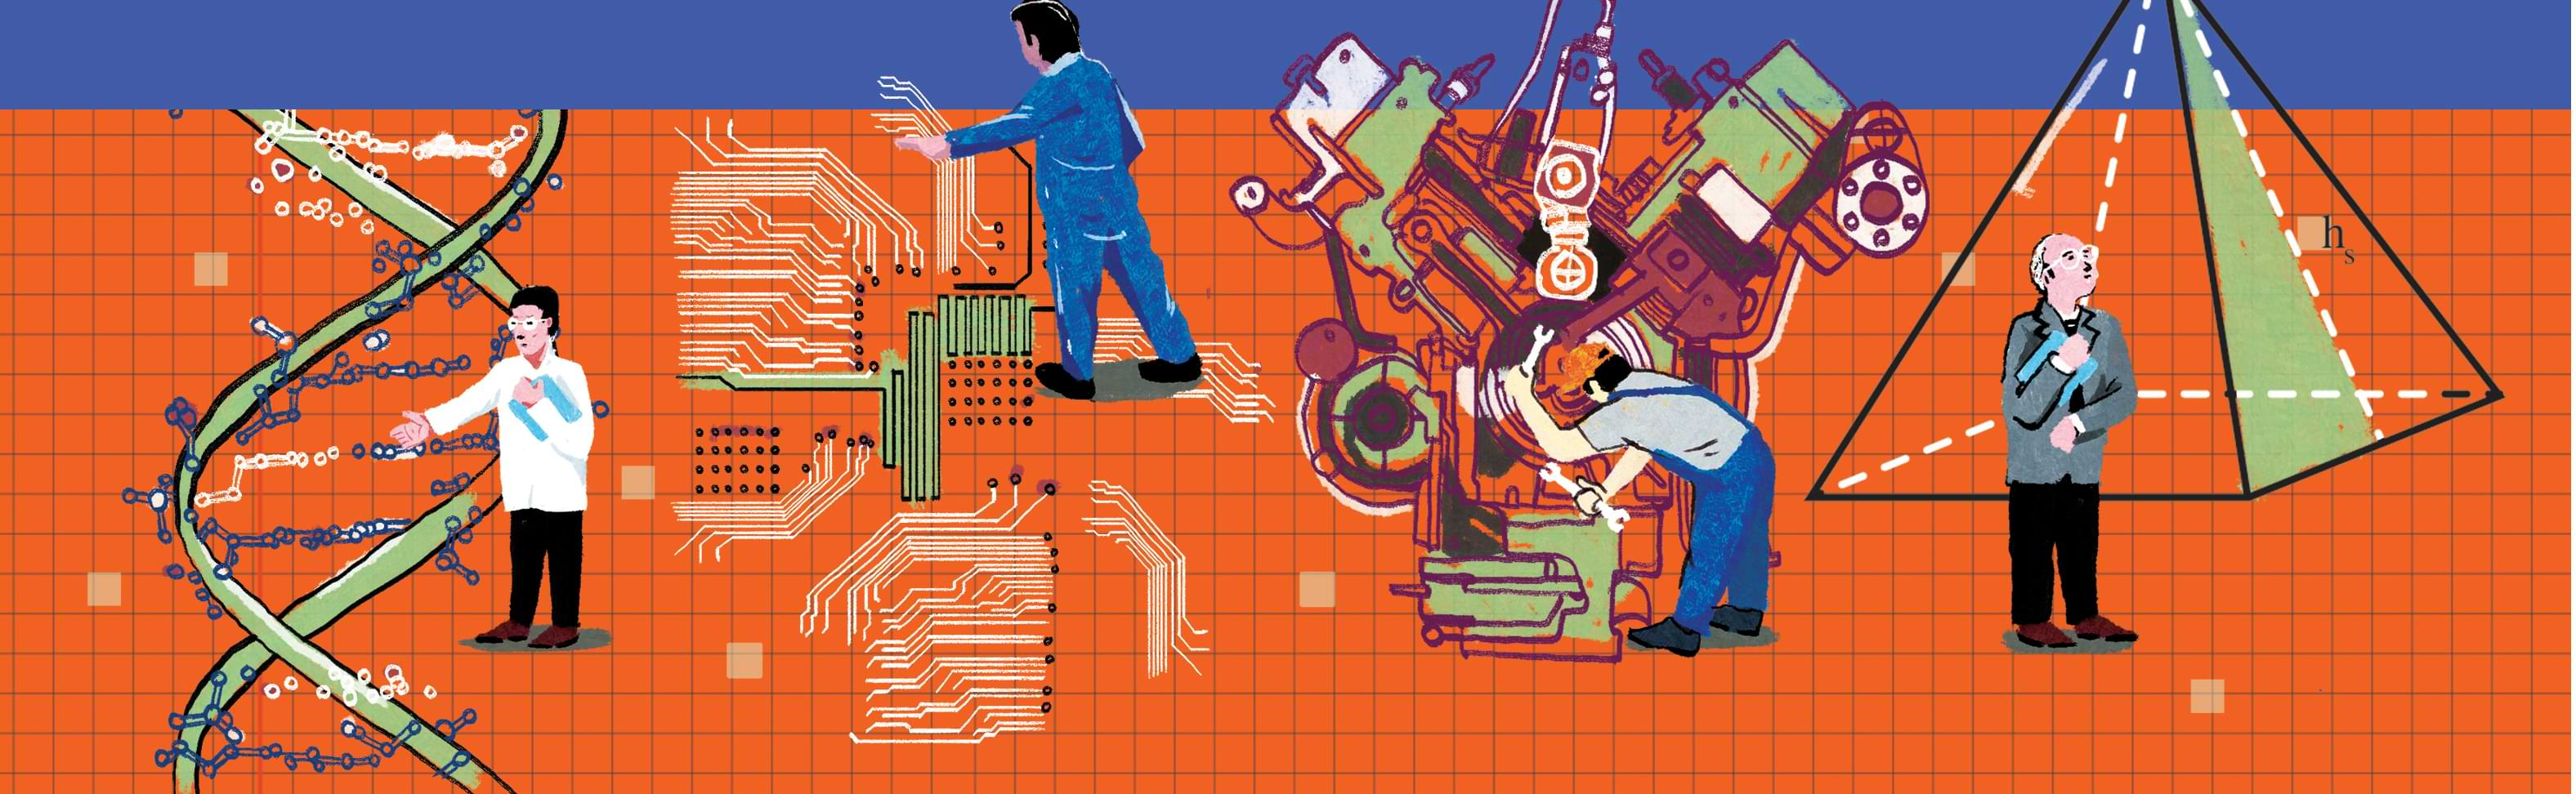
\includegraphics[width=19.3cm]{../bannertimhieu}}}
\AddToShipoutPicture*{\put(130,540){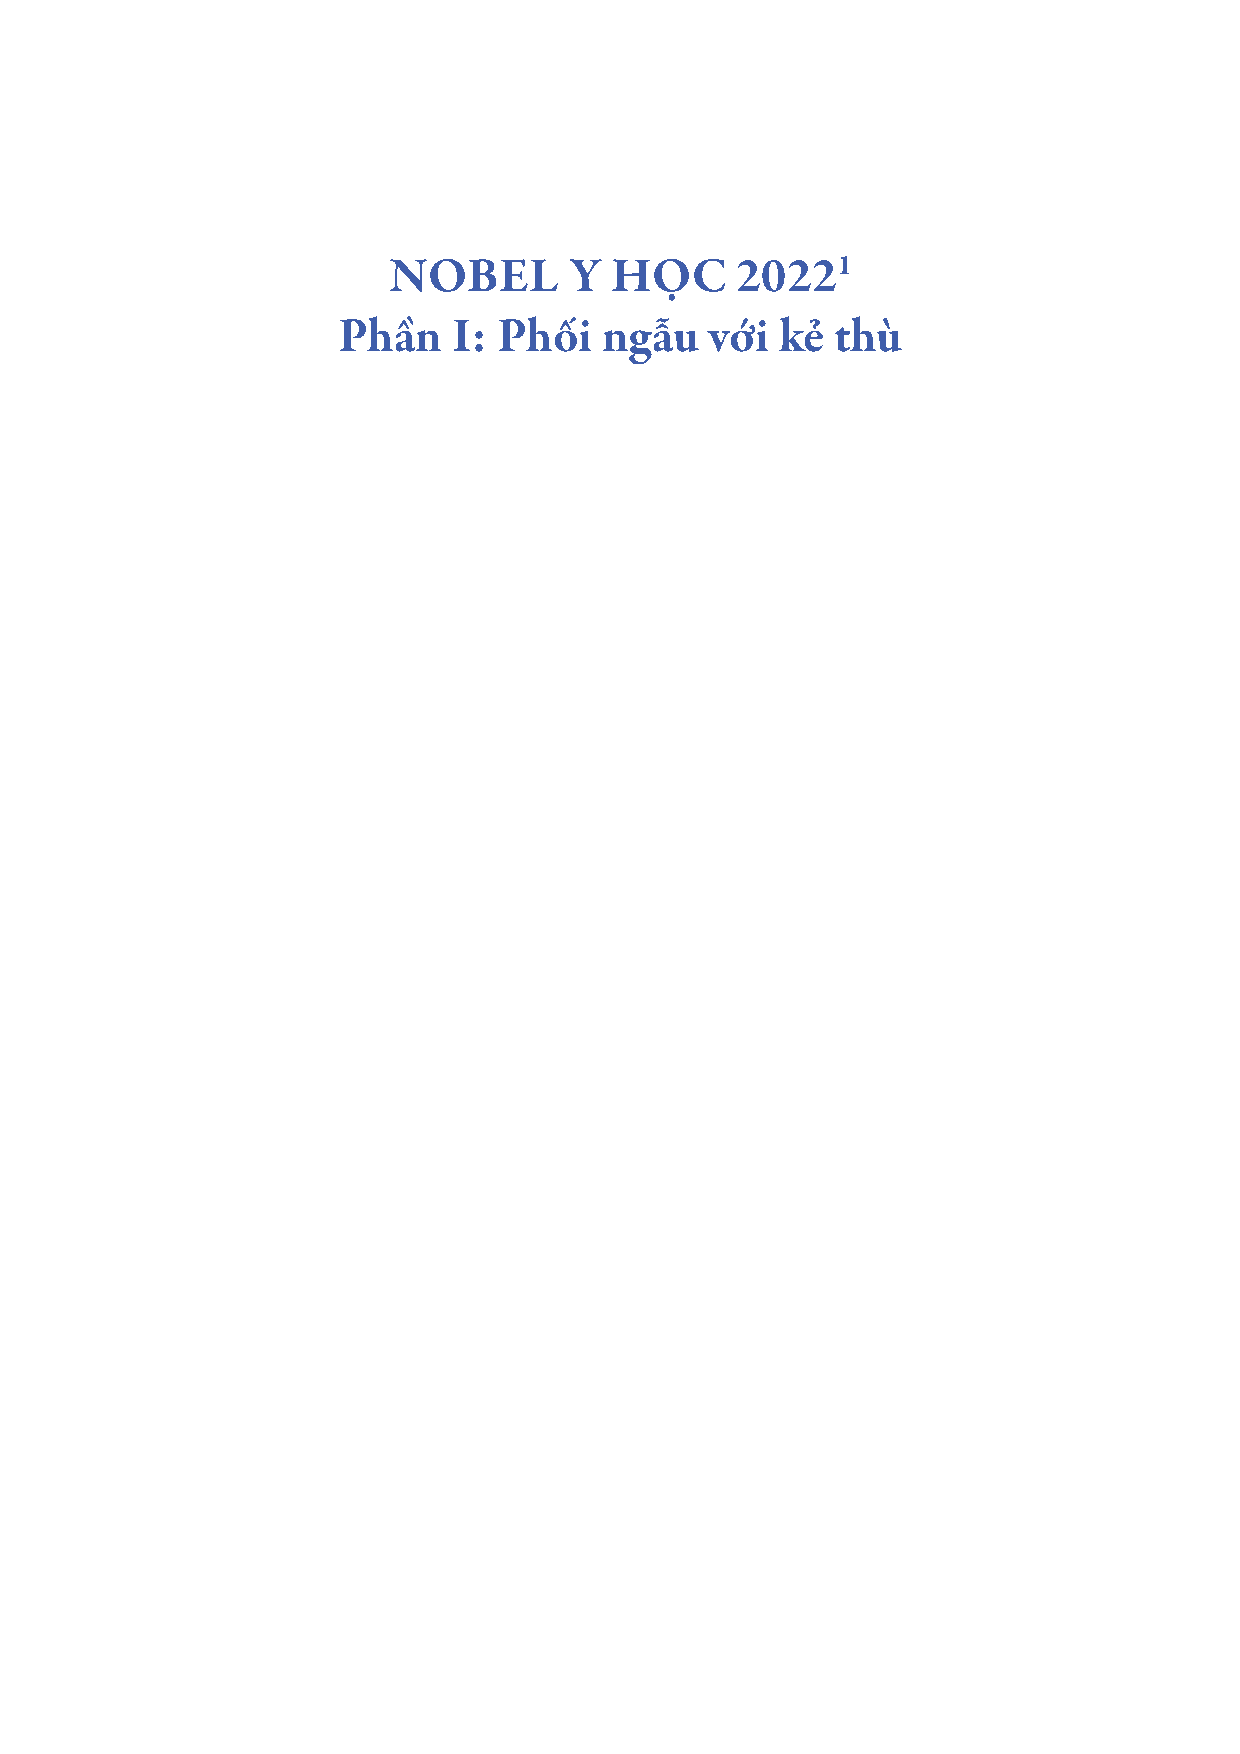
\includegraphics[scale=1]{../tieude.pdf}}}
\centering
\endgroup
\vspace*{160pt}

\begin{multicols}{2}
	Vào đầu tháng $10$ vừa qua, Svante Pääbo được trao giải Nobel Y học “vì những khám phá liên quan đến hệ gene của những nhóm người đã tuyệt chủng và liên quan đến sự tiến hóa của loài người”. Bài viết dưới đây, được đăng trên tạp chí The New Yorker năm $2011$, không lâu sau khi ông công bố bản thảo trình tự hệ gene của người Neanderthal trên Tạp chí Science, làm chấn động thế giới, kể lại hành trình nghiên cứu vừa kỳ lạ, vừa thăng hoa của ông.  
	\begin{figure}[H]
		\vspace*{-5pt}
		\centering
		\captionsetup{labelformat= empty, justification=centering}
		
\includegraphics[width= 1\linewidth]{1}
		\caption{\small\textit{\color{timhieukhoahoc}Người Neanderthal. \\Ảnh: Atelier Daynès và S. Entressangle.}}
		\vspace*{-10pt}
	\end{figure}
	\textbf{\color{timhieukhoahoc}Điều gì đã xảy ra giữa chúng ta và những người Neanderthal?}
	\vskip 0.1cm
	Svante Pääbo là người đứng đầu bộ phận di truyền tiến hóa của Viện Max Planck về Nhân chủng Tiến hóa, Leipzig. Ông cao lêu nghêu, khuôn mặt dài, cằm hẹp và có chòm lông mày rậm thường nhướn lên mỗi khi nhấn mạnh một điều gì trái khoáy. Nổi bật trong văn phòng của Pääbo là mô hình bộ xương người Neanderthal kích thước thật, được dựng thẳng đứng lên khiến đôi bàn chân như đang lơ lửng trên mặt đất, và bức chân dung, lớn hơn cả khổ người Pääbo do sinh viên cao học tặng ông vào dịp sinh nhật lần thứ $50$. Mỗi sinh viên vẽ một mảnh của bức tranh và khi ghép lại cho ra một kết quả giống Pääbo một cách kinh ngạc, chỉ mỗi tội là màu sắc không đồng đều khiến chân dung ông trông như bị mắc bệnh ngoài da.
	\vskip 0.1cm
	Dự án tham vọng nhất của Pääbo cho đến nay là tập hợp một nhóm quốc tế để giải trình tự toàn bộ bộ gene của người Neanderthal. Dự án đang hoàn thành một nửa và đã mang lại một số kết quả chưa chắc chắn lắm, bao gồm những tin tức mà Pääbo tung ra vào năm ngoài, đó là người hiện đại, trước khi diệt chủng người Neanderthal, đã giao phối với họ.
	\vskip 0.1cm
	Nếu bộ gene của người Neanderthal được giải trình hoàn chỉnh thì các nhà khoa học có thể đối chiếu từng gene một, từng cặp base một của họ với con người và xem chúng gặp nhau và rẽ nhánh ở đâu. Đến lúc đó, Pääbo tin rằng, câu trả lời cho trăn trở xa xưa sẽ hoàn toàn trong tầm tay.
	\vskip 0.1cm
	Người Neanderthal có quan hệ rất gần gũi với người hiện đại -- gần đến mức từng đầu gối tay ấp -- và rõ ràng họ không phải con người. Đâu đó nằm giữa những cặp gene khác biệt phải là những đột biến, hay có thể, là những đột biến đã định hình con người chúng ta. Pääbo đã cho một nhóm rà soát hai hệ gene và liệt kê ra những đoạn gene có câu trả lời tiềm năng.
	\vskip 0.1cm
	Pääbo lớn lên ở Stockholm. Mẹ của ông là một nhà hóa học, một người tị nạn Estonia. Bà từng làm việc trong phòng thí nghiệm của nhà hóa sinh Sune Bergström, sau này đã đoạt giải Nobel Y học vào năm $1982$. Pääbo là sản phẩm của một cuộc tình trong phòng thí nghiệm giữa hai người. Mặc dù Pääbo biết cha mình là ai nhưng ông không muốn nhắc đến. Bergström đã có vợ và một con trai khác trong khi mẹ của Pääbo thì chưa bao giờ kết hôn. Vào mỗi thứ bảy, Bergström sẽ đến thăm Pääbo và đưa cậu đi dạo trong rừng hoặc ở một nơi nào khác mà không ai có thể nhận ra ông.
	\vskip 0.1cm
	“Ở nhà coi như ông đi làm vào Thứ Bảy” Pääbo nói với tôi. “Thực sự là việc điên rồ. Vợ ông ấy biết nhưng họ chưa bao giờ nói về nó. Bà không bao giờ gọi cho ông ấy ở nơi làm việc vào các ngày thứ Bảy”. Khi còn nhỏ, Pääbo không đặc biệt bận tâm đến sự sắp xếp này, nhưng sau đó thỉnh thoảng cậu dọa sẽ đến gõ cửa nhà Bergström. “Tôi nói ‘Bố phải nói với con trai của bố vì một lúc nào đó cậu ấy sẽ phát hiện ra’”, ông nhớ lại. Bergström hứa sẽ làm nhưng không bao giờ thực hiện. (Kết quả là người con trai khác của Bergström không biết đến sự tồn tại của Pääbo cho đến trước khi Bergström qua đời vào năm $2004$ không lâu).
	\vskip 0.1cm
	\textbf{\color{timhieukhoahoc}Nghiên cứu bí mật}
	\vskip 0.1cm
	Ngay từ khi còn nhỏ, Pääbo đã thích thú với những thứ cổ cổ. Anh ta phát hiện ra xung quanh những cây đại thụ bị bật gốc có thể tìm thấy những mảnh gốm của người Thụy Điển thời tiền sử, và mang về để đầy căn phòng của mình. Thời thiếu niên một lần được mẹ đưa đến thăm các Kim tự tháp, ông đã bị nó mê hoặc nên sau đó đã đăng ký học Đại học Uppsala và dự định trở thành một nhà Ai Cập học. “Tôi thực sự muốn khám phá những xác ướp, giống như Indiana Jones,” ông nói. Tuy nhiên hầu hết các môn học đều liên quan đến việc phân tích chữ tượng hình, thay vì cảm thấy kích thích thì Pääbo nghĩ nó thật nhàm chán. Được truyền cảm hứng từ cha mình, ông chuyển sang học Y rồi sau đó là Sinh học tế bào.
	\vskip 0.2cm
	\PIbox{“Điều gì đã khiến chúng ta có thể xây dựng nên những xã hội to lớn này, tỏa ra toàn cầu và phát triển công nghệ mà tôi nghĩ không ai có thể nghi ngờ, là năng lực độc nhất của con người. Phải có một cơ sở di truyền cho điều đó, và nó đang ẩn náu đâu đó trong những đoạn gene này”.
	\vskip 0.1cm
	\hfill \textit{Svante Pääbo}}
	\vskip 0.2cm
	Vào đầu những năm $1980$, khi Pääbo đang làm nghiên cứu sinh về virus thì đột nhiên ông lại mơ tưởng đến xác ướp một lần nữa. Ít nhất là theo hiểu biết của ông lúc bấy giờ, chưa ai tìm cách lấy DNA từ những xác chết cổ đại. Ông tự dưng cảm thấy điều đó là khả thi, và thế là một phương pháp nghiên cứu lịch sử hoàn toàn mới ra đời.
	\vskip 0.1cm
	Sợ rằng thầy hướng dẫn sẽ bảo ý tưởng này là ngớ ngẩn (hoặc tệ hơn thế) nên Pääbo đã bí mật tiến hành nghiên cứu xác ướp, vào ban đêm. Nhờ quen một giáo sư Ai Cập học, ông đã tìm được một số mẫu vật từ Bảo tàng Ai Cập ở Đông Berlin. Năm $1984$, ông công bố kết quả của mình trên một tạp chí Đông Đức ít người biết đến. Ông công bố đã phát hiện được DNA trong tế bào của một đứa trẻ được ướp xác đã chết hơn $2{.}000$ năm. Pääbo kỳ vọng có thể tìm được lời giải đáp cho những câu hỏi như điều gì đã khiến các triều đại Pharaon thay đổi và mẹ của Tutankhamun là ai từ DNA của các xác ướp này.
	\vskip 0.1cm
	Trong lúc soạn thảo phiên bản tiếng Anh của bài báo thì một nhóm các nhà khoa học Đại học California tại Berkeley thông báo rằng họ đã thành công trong việc giải trình tự một đoạn DNA từ một động vật giống ngựa vằn được gọi là quagga, một loài thú đã bị săn bắn đến tuyệt chủng vào những năm $1880$. (DNA này được lấy từ xác con thú hơn $140$ năm tuổi được bảo quản tại Bảo tàng Lịch sử Quốc gia Mainz). Trưởng nhóm Berkeley, Allan Wilson là một nhà hóa sinh có tiếng tăm. Ông là người tìm ra phương pháp nghiên cứu sự tiến hóa sử dụng khái niệm “đồng hồ phân tử”. Pääbo liền gửi cho Wilson một số đoạn trong bài báo xác ướp của mình. Wilson rất ấn tượng và ngỏ ý hỏi có còn vị trí nào trống trong lab của Pääbo; ông muốn dành kỳ  sabbatical  (nghỉ phép để nghiên cứu) ở đó. Pääbo trả lời Wilson rằng mình không thể cho Wilson một vị trí nào ở phòng lab cả, vì đáng tiếc là anh nào có lab đâu -- thậm chí lúc đó còn chưa có bằng tiến sỹ nữa kìa.
	\begin{figure}[H]
		\vspace*{-5pt}
		\centering
		\captionsetup{labelformat= empty, justification=centering}
		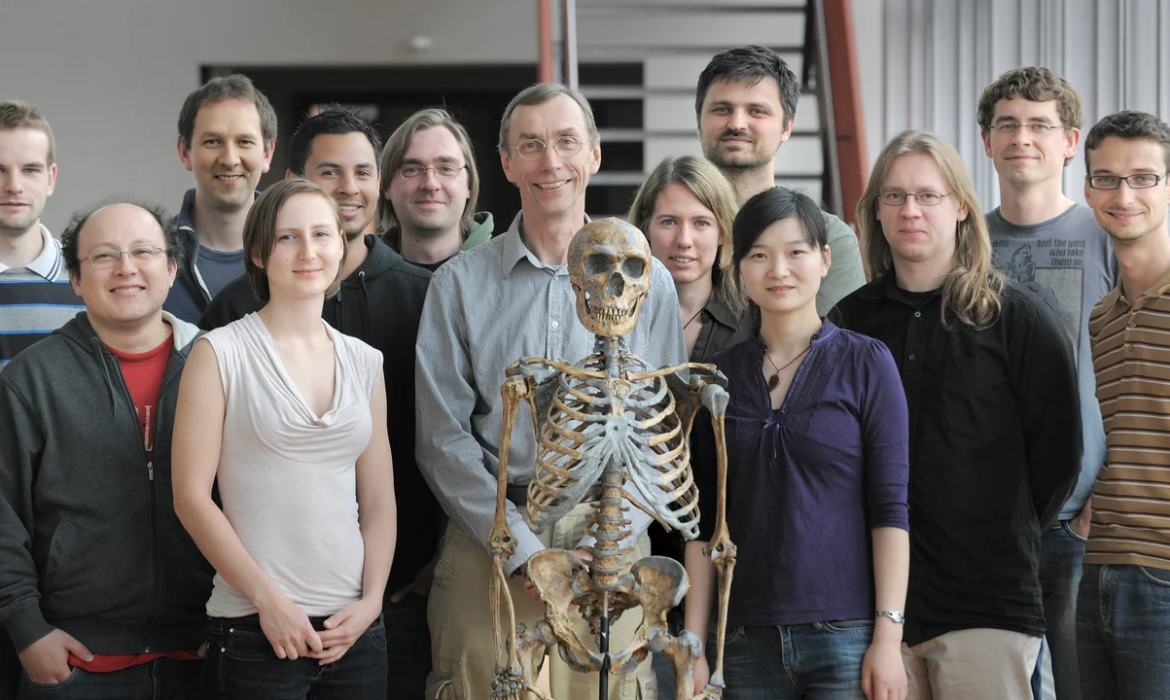
\includegraphics[width= 1\linewidth]{2}
		\caption{\small\textit{\color{timhieukhoahoc}Nhóm nghiên cứu của Svante Pääbo. \\Ảnh: mpg.de}}
		\vspace*{-10pt}
	\end{figure}
	Bài báo về xác ướp của Pääbo được công bố trên trang bìa tạp chí \textit{Nature}. Tờ \textit{New York Times} còn viết về nó, gọi đây là “công trình kịch tính nhất trong một loạt các thành tựu gần đây của sinh học phân tử”. Dẫu vậy, các đồng nghiệp của Pääbo ở Thụy Điển vẫn tỏ ra hoài nghi. Họ giục ông hãy quên đi những xác chết nhăn nheo và kiên định với virus. “Tất cả nọi người đều nói với tôi rằng thật là ngu xuẩn khi rời bỏ một lĩnh vực quan trọng để đến với một thứ gần giống như trò tiêu khiển”. Pääbo phớt lờ họ, đến Berkeley làm việc cho Wilson.
	\vskip 0.1cm
	\textbf{\color{timhieukhoahoc}Một ngành khoa học mới}
	\vskip 0.1cm
	“Anh ấy lên cứ như diều gặp gió” -- Mary--Claire King, người cũng từng là sinh viên của Wilson và hiện là giáo sư về Hệ gene học tại Đại học Washington, nhớ là Pääbo và Wilson (ông qua đời năm $1991$). “Cả hai đều nghĩ về những ý tưởng rất lớn”. “Và mỗi người đều rất giỏi trong việc chuyển những ý tưởng đó thành những giả thuyết có thể kiểm chứng được. Cả hai cũng rất giỏi trong việc phát triển công nghệ cần thiết để kiểm tra các giả thuyết. Có được cả ba năng lực đó thì quả là đáng nể ”. Ngoài ra,  dù ``cả hai đều rất tôn trọng dữ liệu, không ai ngần ngại nói những điều gây sốc về dữ liệu của mình, và họ đều không hề sợ sai”.
	\vskip 0.1cm
	DNA bao gồm các phân tử được gọi là nucleotide đan lại với nhau theo hình bậc thang -- chính là chuỗi xoắn kép nổi tiếng. Mỗi nucleotide chứa một trong bốn base (bazơ): Adenine, Thymine, Guanine và Cytosine được ký hiệu bằng các chữ cái A, T, G và C. Do đó một đoạn của bộ gene người có thể được biểu thị là ACCTCCTCTAATGTCA. Bộ gene của con người là một dải ba tỷ cặp base. Theo những gì đã xác định đến giờ này, thì phần lớn các cặp base đều không đáng quan tâm.
	\vskip 0.1cm
	Ngoại trừ các tế bào hồng cầu thì mọi tế bào trong một sinh vật đều chứa một bản sao hoàn chỉnh của DNA của nó. Nó cũng chứa nhiều bản sao, từ hàng trăm đến hàng nghìn, của một dạng DNA rút gọn được gọi là DNA ty thể (mtDNA). Nhưng ngay sau khi sinh vật chết thì các chuỗi nucleotide dài bắt đầu bị phá vỡ. Phần lớn diễn ra trong vài giờ đầu tiên bởi các enzym bên trong cơ thể của chính sinh vật. Sau một thời gian, tất cả những gì còn lại là các đoạn mã, và sau một thời gian nữa -- phụ thuộc vào các điều kiện phân hủy -- những đoạn mã này cũng tan rã. “Có lẽ trong lớp băng vĩnh cửu bạn có thể quay ngược lại năm trăm nghìn năm,” Pääbo nói với tôi. “Nhưng chắc chắn trong giới hạn một triệu năm thôi.” Năm trăm nghìn năm trước thì loài khủng long cũng đã tuyệt chủng được hơn $64$ triệu năm nên toàn bộ hình dung về “công viên kỷ Jura”, đáng tiếc, chỉ dừng lại ở tưởng tượng. Thế nhưng, năm trăm nghìn năm trước thì con người hiện đại vẫn chưa ra đời.
	\vskip 0.2cm
	\PIbox{
	“Pääbo đã đưa lĩnh vực nghiên cứu DNA cổ đại, vốn ban đầu chỉ là chuyện giả tưởng trong phim ‘Công viên kỷ Jura’ thành một khoa học thực sự, đó là một thành tựu lớn”.
	\vskip 0.1cm
	\hfill \textit{Maynard Olson}}
	\vskip 0.2cm
	Khi đến California, Pääbo vẫn quan tâm đến hướng sử dụng di truyền học để nghiên cứu lịch sử loài người. Tuy nhiên trong khi cố gắng xác định vị trí các đoạn ADN của người Ai Cập cổ đại, ông đã phát hiện ra một vấn đề lớn: chúng trông rất giống -- thực sự, giống hệt -- các đoạn ADN của con người đương đại. Như vậy phân tử vi mô trên da của ông hoặc của người khác, thậm chí là của giám tuyển bảo tàng đã qua đời từ lâu tình cờ rơi vào, cũng có thể phá hỏng công sức cả tháng trời làm việc.
	\vskip 0.1cm
	Ông giải thích: “Rõ ràng là tạp nhiễm từ bên ngoài là một vấn đề lớn. (Cuối cùng, Pääbo kết luận rằng các trình tự mà mình thu được trong bài báo xác ướp ban đầu của mình có thể đã bị hỏng vì lý do này). Và để khởi động, ông bắt đầu nghiên cứu những loài động vật đã tuyệt chủng. Ông phân tích mẫu mtDNA từ những con lười khổng lồ trên mặt đất đã biến mất khoảng mười hai nghìn năm trước như voi ma mút hay hổ Tasmania, bị săn bắn đến tuyệt chủng vào thập niên $1930$. Ông cũng trích xuất mtDNA từ moas, loài chim khổng lồ không biết bay sống ở New Zealand trước khi người Maori đến, và nhận thấy rằng moas có quan hệ họ hàng gần với các loài chim từ Úc hơn là kiwi, loài chim không bay sống ở New Zealand ngày nay. Ông cũng thăm dò rất nhiều xác sinh vật không có DNA nào hữu ích, như xương từ công viên cổ sinh La Brea (nơi có hàng ngàn sinh vật thời kỳ băng hà bị chôn trong nhựa đường) và côn trùng hóa thạch được bảo quản trong hổ phách. Trong quá trình làm việc này, Pääbo ít nhiều đã phát minh ra lĩnh vực cổ sinh học.
	\vskip 0.1cm
	“Thành thật mà nói đây là vấn đề mà bản thân tôi sẽ không muốn giải quyết, vì tôi nghĩ nó quá khó,” Maynard Olson, giáo sư danh dự tại Đại học Washington và một trong những người sáng lập Dự án Genome người Neanderthal đã nói với tôi. “Pääbo đã mang lại những tiêu chuẩn rất cao cho lĩnh vực này, và đưa lĩnh vực nghiên cứu DNA cổ đại, vốn ban đầu chỉ là chuyện giả tưởng trong phim ‘Công viên kỷ Jura’ thành một khoa học thực sự, đó là một thành tựu lớn”.
	\begin{figure}[H]
		\vspace*{-5pt}
		\centering
		\captionsetup{labelformat= empty, justification=centering}
		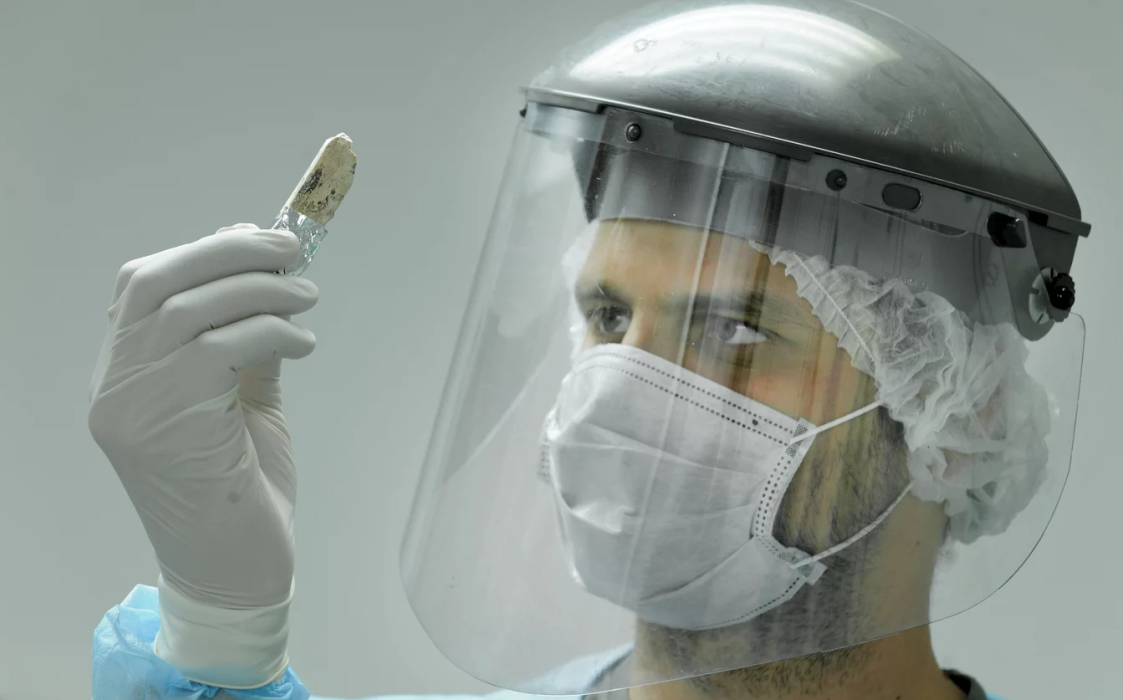
\includegraphics[width= 1\linewidth]{3}
		\caption{\small\textit{\color{timhieukhoahoc}Các nhà nghiên cứu phải rất cẩn trọng để tránh chính DNA của mình làm tạp nhiễm những mẩu xương cổ đại.}}
		\vspace*{-10pt}
	\end{figure}
	Ed Green, giáo sư kỹ thuật phân tử sinh học tại Đại học California ở Santa Cruz, người làm việc trong Dự án bộ Gene người Neanderthal cho biết: “Hầu hết các ngành khoa học đều không có gì đặc biệt. Nếu bạn không làm, thì vài tháng sau sẽ có người khác làm về lĩnh vực đó. Svante là một trong số những nhà khoa học hiếm hoi chứng minh điều ngược lại. Nếu không có ông, sẽ không có ngành DNA cổ đại như chúng ta đã biết”.
	\vskip 0.1cm
	\textbf{\color{timhieukhoahoc}Bước ngoặt trong nghiên cứu}
	\vskip 0.1cm
	Đại học Munich đã đề nghị Pääbo làm trợ lý giáo sư. Vì không có lý do thúc ép nào để chuyển đến Đức nên ông do dự. Rồi đề nghị đó trở thành lời mời làm giáo sư toàn phần: “Và rồi tôi nói, ồ chắc nước Đức cũng không tệ lắm đâu. Tôi sẽ đến đó vài năm”.
	\vskip 0.1cm
	Khi bảo tàng Bang Rhenish, ở Bonn gọi Pääbo nhiều năm sau đó, ông vẫn đang yên vị ở Munich. Bảo tàng này lưu giữ xương của người Neanderthal đầu tiên được xác định, được phát hiện vào mùa hè năm $1856$. Ông nghĩ mình có bao bao nhiêu $\%$ cơ hội để trích xuất những DNA hữu ích từ đó? Pääbo chỉ có thể xác định được tình trạng những chiếc xương cho đến khi ông tìm đến chúng.
	\vskip 0.1cm
	“Tôi không biết phải nói gì với họ, vì vậy tôi nói,” Có $5\%$ cơ hội có thể tìm ra”, ông nhớ lại. Vài tháng sau, ông nhận được một phần nhỏ của hài cốt bên phải của người Neanderthal.
	\vskip 0.1cm
	Người Neanderthal đầu tiên được tìm thấy trong một hang động đá vôi cách Bonn khoảng bốn mươi lăm dặm về phía Bắc, trong một khu vực được gọi là Thung lũng Neander, theo tiếng Đức là das Neandertal. Mặc dù hang động đã biến mất -- đá vôi từ lâu đã được khai thác để phục vụ xây dựng -- khu vực này bây giờ là một công viên giải trí theo chủ đề người Neanderthal với bảo tàng riêng, những con đường mòn đi bộ đường dài và một khu vườn trồng các loại cây bụi đã xuất hiện từ kỷ băng hà. Người Neanderthal ở đây được khắc họa như những con người dễ mến, nếu không muốn nói là cuốn hút. Lối vào tòa nhà là một mô hình người Neanderthal cao tuổi đang chống gậy. Bên cạnh ông ta là một trong những điểm tham quan nổi tiếng nhất của bảo tàng -- một phòng chụp ảnh tên là Morphing-Station. Với $3$ euro, khách đến đây sẽ được nhận một bức ảnh chụp chân dung họ bình thường, một bức ảnh thứ hai, đối xứng với bức thứ nhất, được chỉnh sửa với cằm thụt vào trong, trán hếch và sau đầu phồng ra. Lũ trẻ thích tự nhìn mình -- hay đặc biệt là chứng kiến anh chị em chúng -- bị biến hình thành người Neanderthal. Chúng thấy buồn cười kinh lên được.
	\vskip 0.1cm
	Những bộ xương đầu tiên của người Neanderthal xuất hiện ở Thung lũng Neander bị đối xử như rác rưởi. Các mảnh vỡ như nắp sọ, bốn xương cánh tay, hai xương đùi và một phần xương chậu, về sau được một doanh nhân địa phương thu vén lại. Anh ta lại nghĩ rằng đó là xương của một con gấu tiền sử và gửi đến cho một người sưu tập hóa thạch. Người thu thập hóa thạch nhận ra rằng đây là một thứ lạ lẫm hơn nhiều so với một con gấu, một “thành viên nguyên thủy của chủng tộc chúng ta”.
	\vskip 0.1cm
	\PIbox{
	Trước khi Neanderthal bị ``thay thế", họ và người hiện đại đã có những hậu duệ chung, trở thành những công dân của châu Âu, châu Á và Tân Thế giới.}
	\vskip 0.1cm
	Và rồi điều này xảy ra đúng vào khoảng thời gian Darwin xuất bản cuốn “Về nguồn gốc của các loài”, và các mảnh xương nhanh chóng trở thành chủ đề tranh luận về nguồn gốc của con người. Những người phản đối thuyết tiến hóa khăng khăng rằng chúng thuộc về một người bình thường. Một giả thuyết cho rằng đó là một người Cossack đã lưu lạc đến khu vực trong cuộc hỗn loạn sau Chiến tranh Napoléon. Lý do bộ xương trông kỳ lạ -- xương đùi của người Neanderthal bị cong một cách đặc trưng -- là người Cossack đã ngồi quá lâu trên ngựa. Một người khác cho rằng hài cốt là của một người đàn ông bị bệnh còi xương: người đàn ông này đã phải chịu đựng quá nhiều cơn đau vì căn bệnh của mình đến mức khiến trán của anh ta luôn căng ra -- do đó, một phần xương trán bị nhô ra. (Nhưng không ai thấy phân vân khi một người đã còi xương và thường xuyên đau đớn lại leo trèo vào hang động làm~gì).
	\vskip 0.1cm
	Trong những thập kỷ tiếp theo, những bộ xương giống xương của người ở Thung lũng Neander -- dày hơn xương của người hiện đại, với những hộp sọ có hình dạng kỳ lạ -- đã được phát hiện tại một số địa điểm khác bao gồm hai ở Bỉ và một ở Pháp. Trong khi đó một hộp sọ được khai quật nhiều năm trước đó ở Gibraltar được cho là trông rất giống với hộp sọ tìm thấy ở Đức. Rõ ràng tất cả những thứ còn sót lại này không thể được giải thích bằng chuyện về người Cossack lạc đường hay người còi xương đi thám hiểm hang động nữa. Nhưng các nhà tiến hóa cũng không biết giải thích thế nào. Người Neanderthal có hộp sọ rất lớn -- trung bình lớn hơn người hiện đại ngày nay. Điều này khiến chúng ta khó có thể đưa họ vào trong quá trình tiến hóa từ loài vượn có não nhỏ tiến lên những bộ não lớn hơn cho đến con người. Trong cuốn “Hậu duệ của con người” xuất bản năm $1871$, Darwin chỉ đề cập đến người Neanderthal rất ngắn. “Phải thừa nhận rằng một số hộp sọ có tính rất cổ xưa, chẳng hạn như hộp sọ nổi tiếng của người Neanderthal, đã phát triển tốt và có năng lực,” ông lưu ý.
	\vskip 0.1cm
	Năm $1908$, một bộ xương gần như hoàn chỉnh của người Neanderthal được phát hiện trong một hang động gần La Chapelle--aux--Saints, miền Nam nước Pháp. Bộ xương đã được gửi đến một nhà cổ sinh vật học tên là Marcellin Boule thuộc Bảo tàng Lịch sử Tự nhiên Quốc gia Paris. Trong một loạt sách chuyên khảo, Boule đã phát minh ra thứ tạm gọi là bức biếm họa về người Neanderthal -- đầu gối cong, lưng gù và tàn bạo. Boule viết: các xương của người Neanderthal thể hiện một “cấu trúc linh trưởng đặc trưng”, và hình dạng hộp sọ cho thấy đây là “một loài kém phát triển hoặc hung tợn”. Các kết luận của Boule được nhiều người cùng thời với ông nghiên cứu và lặp lại; Ví dụ, nhà nhân chủng học người Anh, Sir Grafton Elliot Smith, đã mô tả người Neanderthal đi đứng với “một cơ thể khùng khoằm” đặt trên “một đôi chân đặc biệt dị dạng” (Smith còn mô tả người Neanderthal thêm muôn phần xấu xí với gần như toàn thân lông lá dù đến nay chưa hề có bằng chứng rõ ràng nào cho thấy họ nhiều lông).
	\vskip 0.1cm
	Vào những năm $1950$, hai nhà giải phẫu học Williams Straus và Alexander Cave quyết định kiểm tra lại bộ xương từ La Chapelle. Straus và Cave khẳng định rằng những gì Boule tưởng là dáng đi tự nhiên của người Neanderthal, thực ra là do bệnh viêm khớp. Người Neanderthal không đi bộ với tư thế còng lưng và khuỵu chân. Thật vậy, nếu cạo râu nhẵn nhụi và khoác một bộ cánh mới và bước vào tàu điện ngầm ở New York thì một người Neanderthal có lẽ sẽ chả khiến ai chú ý “hơn một số cư dân khác của thành phố này”, họ viết. Nhiều nghiên cứu gần đây có xu hướng ủng hộ ý tưởng như vậy.
	\vskip 0.1cm
	Pääbo quyết định giải trình tự toàn bộ hệ gene của người Neanderthal vào tháng $7/2006$ đúng vào dịp kỷ niệm $155$ năm phát hiện ra người Neanderthal. Thông báo được đưa ra cùng với một công ty của Mỹ, $454$ Life Sciences, công ty đã phát triển một máy giải trình tự “thông lượng cao” với sự trợ giúp của các quả cầu nhựa nhỏ, có thể tái tạo hàng chục nghìn đoạn DNA cùng một lúc. Cả trong và ngoài ngành di truyền học kế hoạch này được xem là vô cùng tham vọng và dự án đã gây tiếng vang trên toàn thế giới. “Một nghiên cứu thật to gan”, tiêu đề trên tờ \textit{The Economist} tuyên bố.
	\vskip 0.1cm
	\textbf{\color{timhieukhoahoc}Con đường chông gai}
	\vskip 0.1cm
	Giờ đây, một phiên bản hoàn chỉnh của bộ gene người đã được công bố. Cùng với đó là các phiên bản hệ gene khác của tinh tinh, chuột, chuột cống cũng hoàn thành. Nhưng con người, tinh tinh, chuột và chuột cống đều là sinh vật sống, trong khi người Neanderthal đã tuyệt chủng trong ba mươi nghìn năm. Rào cản đầu tiên chỉ đơn giản là tìm đủ DNA của người Neanderthal để giải trình tự. Mẫu vật còn lại của người Neanderthal mà Pääbo nhận được ban đầu đã mang lại một số thông tin di truyền nhưng còn xa mới đủ số lượng cần thiết để lắp ráp/tập hợp lại cho đủ toàn bộ bộ gene. Vì vậy, Pääbo đã đặt hy vọng của mình vào một nhóm xương khác từ Croatia. (Xương của người Croatia hóa ra thuộc về ba người, tất cả đều là phụ nữ; người Neanderthal ban đầu có lẽ là đàn ông).
	\vskip 0.1cm
	Đến cuối năm $2006$, Pääbo và nhóm của ông báo cáo rằng bằng cách sử dụng một mảnh xương của người Croatia, họ đã thành công trong việc giải trình tự một triệu cặp base của bộ gene người Neanderthal. (Cũng giống như bộ gene của con người, bộ gen đầy đủ của người Neanderthal bao gồm khoảng ba tỷ cặp cơ bản). Ngoại suy ra họ ước tính sẽ mất khoảng hai năm và sáu nghìn lần “chạy” trên một cỗ máy $454$ Life Sciences để hoàn thành dự án. Nhưng phân tích sau đó cho thấy hàng triệu cặp base có thể đã bị tạp nhiễm bởi DNA của con người. Điều này khiến một số nhà di truyền học đặt câu hỏi liệu Pääbo có vội vàng công bố những kết quả mà lẽ ra anh ta phải biết là sai hay không. Trong khi đó, các xương tiếp theo mang lại tỷ lệ DNA Neanderthal thấp hơn nhiều và tỷ lệ DNA vi sinh vật cao hơn nhiều. (Khoảng $80\%$ DNA đã giải trình tự trong Dự án bộ gene người Neanderthal đều thuộc về vi sinh vật và, theo dự án thì hoàn toàn là vô dụng). Điều này có nghĩa là, công sức để hoàn thiện bộ gene lớn hơn rất nhiều so với những ước tính ban đầu. “Đã có những lúc tuyệt vọng,” Pääbo nói với tôi. Giải quyết được vấn đề này thì lại nảy ra vấn đề khác. “Đó là một chuyến tàu lượn đầy cảm xúc,” Ed Green, kỹ sư phân tử sinh học từ Santa Cruz, nhớ lại.
	\vskip 0.1cm
	Khoảng sau hai năm bắt đầu dự án, một thách thức nảy sinh. Pääbo đã tập hợp một nhóm quốc tế để giúp phân tích dữ liệu từ các máy giải trình tự -- về cơ bản, là một danh sách dài của A, T, G, C. Đang sàng lọc dữ liệu thì một trong những thành viên của nhóm, David Reich, một nhà di truyền học tại Trường Y Harvard, đã nhận thấy điều kỳ lạ. Trình tự của người Neanderthal, đúng như dự đoán, rất giống với trình tự của con người. Nhưng có những kiểu người giống với người Neanderthan hơn những kiểu người khác. Cụ thể, người châu Âu và châu Á chia sẻ DNA với người Neanderthal nhiều hơn người châu Phi. “Chúng tôi đã cố gắng phủ nhận kết quả này”, Reich nói với tôi. “Chúng tôi đã nghĩ, không thể thế~được”.
	\vskip 0.1cm
	Trong khoảng $25$ năm qua, nghiên cứu về sự tiến hóa của loài người đã bị chi phối bởi lý thuyết được báo chí đại chúng gọi là “Từ châu Phi mà ra” (Out of Africa), hay giới học thuật gọi là giả thuyết “nguồn gốc duy nhất gần đây” hoặc giả thuyết “thay thế”. Lý thuyết này cho rằng tất cả con người hiện đại đều là hậu duệ của một nhóm dân số nhỏ sống ở châu Phi khoảng hai trăm nghìn năm trước. (Không lâu trước khi ông qua đời, Allan Wilson, cố vấn của Pääbo đã phát triển một trong những bằng chứng quan trọng cho lý thuyết, dựa trên sự so sánh DNA ty thể của người đương đại). Khoảng một trăm hai mươi nghìn năm trước một nhóm nhỏ người đã di cư vào Trung Đông, và đến năm mươi nghìn năm trước, một nhóm con khác đã đi vào lục địa Âu--Á. Khi di chuyển về phía Bắc và phía Đông, con người hiện đại chạm trán với người Neanderthal và những người khác được gọi là “người cổ đại”, những người đã sinh sống ở những vùng này trước đó. Con người hiện đại đã “thay thế” con “người cổ đại”, thật là một xảo ngôn che giấu việc con người đã đẩy họ đến tuyệt chủng. Mô hình di cư và “thay thế” này ngụ ý rằng dù đến từ đâu thì con người và người Neanderthal cũng có mối quan hệ (thù địch) với nhau.
	\vskip 0.1cm
	Nhiều thành viên trong nhóm của Pääbo những tưởng đó là một trường hợp nhiễm tạp khác. Nhiều khi các mẫu xử lý bởi người châu Âu; đã bị trộn DNA của họ với DNA của người Neanderthal. Người ta đã chạy một số thử nghiệm để đánh giá khả năng này. Các kết quả đều âm tính. Reich nói với tôi: “Chúng tôi tiếp tục nhìn thấy đặc tính này và càng có nhiều dữ liệu xác nhận nó về mặt thống kê. Dần dần, các thành viên khác trong nhóm bắt đầu suy nghĩ. Trong một bài báo đăng trên tạp chí \textit{Science}, vào tháng $5/2010$, họ đã giới thiệu điều mà Pääbo gọi là giả thuyết “thay thế bị rò rỉ”. (Bài báo sau đó được bình chọn là bài báo xuất sắc của năm và nhóm nghiên cứu đã nhận được giải thưởng $25$ nghìn USD).
	\vskip 0.1cm
	Giả thuyết “thay thế bị rò rỉ” -- giả định rằng nó đúng vào lúc này -- cung cấp thêm bằng chứng về sự gần gũi của người Neanderthal với con người hiện đại. Không chỉ cả hai đã giao phối với nhau, mà những đứa con lai cũng đủ cứng cáp để hòa nhập vào xã hội loài người. Một số con lai này sống sót để có những đứa con của riêng mình, đến lượt chúng, lại sinh con, và cứ thế cho đến ngày nay. Ngay cả bây giờ, ít nhất là ba mươi nghìn năm sau sự kiện này, tín hiệu này vẫn không thể khiến chúng ta làm ngơ: tất cả những người không có nguồn gốc châu Phi, từ người New Guinea đến người Pháp cho đến người Hán Trung Hoa đều mang đâu đó từ một đến bốn phần trăm DNA của người Neanderthal.
	\vskip 0.1cm
	Khi cuối cùng Pääbo có thể đón nhận ý tưởng rằng, người Neanderthal trao lại một số gene của họ cho người hiện đại, ông nói với tôi, “Tôi nghĩ điều đó thật “cool”. Nó có nghĩa là họ không hoàn toàn bị tuyệt chủng -- mà vẫn còn hiện hữu phảng phất trong cơ thể chúng ta”. 
	\vskip 0.1cm
	\hfill\textit{(còn tiếp)}
	\vskip 0.1cm
	\hfill Nguyễn Quang \textit{dịch}\footnote[2]{\color{timhieukhoahoc} Nguyên tác: https://www.newyorker.com/magazine/2011/08/15/sleeping-with-the-enemy}
\end{multicols}
\vspace*{-10pt}
{\color{timhieukhoahoc}\rule{1\linewidth}{0.1pt}}
\vskip 0.2cm
{\centerline{\LARGE\textbf{\color{timhieukhoahoc}LỜI GIẢI, ĐÁP ÁN}}}
\begin{multicols}{2}
	\textbf{\color{timhieukhoahoc}Đố vui}
	\vskip 0.1cm
	$7^2= 49$
	\vskip 0.1cm
	\textbf{\color{timhieukhoahoc}Góc cờ}
	\vskip 0.1cm
	Hình $4$: $\pmb{1)}$ C$5-6$ M$7/5$\quad $\pmb{2)}$ C$6.1$ T$3/5$\quad $\pmb{3)}$ C$2-3$ C$6-5$ \quad $\pmb{4)}$ Tg$5-4$ M$5.7$\quad $\pmb{5)}$ X$5-3$ C$5.1$\quad $\pmb{6)}$ Tg$4.1$ C$4-5$\quad $\pmb{7)}$ Tg$4-5$ C$7.1$ ($1/2$)
	\vskip 0.1cm
	Hình $5$:$\pmb{1)}$ X$4-5$ Tg$5.1$\quad $\pmb{2)}$ C$7-6$ X$4/1$\quad $\pmb{3)}$ C$4.1$ Tg$5/1$\quad $\pmb{4)}$ P$7.8$ S$4.5$\quad $\pmb{5)}$ C$4.1$ S$5/6$\quad $\pmb{6)}$ P$7-4$ Tg$5.1$\quad $\pmb{7)}$ X$8-5$ Tg$5/1$\quad $\pmb{8)}$ P$4-1$ Tg$5.1$\quad $\pmb{9)}$ P$1/1$ Tg$5/1$\quad $\pmb{10)}$ P$1-6$ Tg$5-4$ ($1/2$).
	\vskip 0.1cm
	\textbf{\color{timhieukhoahoc}Thành phố của các công dân thông minh}
	\vskip 0.1cm
	Tất cả các người ngốc ngếch đều trả lời “Một”. Nếu trong tòa thị chính  có ít nhất là $3$ công dân thông minh, thì tất cả họ sẽ đưa ra một số không nhỏ hơn $2$, và Xuân Phong đã biết được ngay câu trả lời. Vì thế, số công dân thông minh chỉ có thể là $0$, $1$ hoặc $2$. Ta xét tất cả các trường hợp.
	\vskip 0.1cm
	Nếu không có công dân thông mình nào, thì tất cả sẽ trả lời là “Một”. Nếu chỉ có một công dân thông minh và hơn nữa lại tự tin, thì anh ta cũng trả lời “Một” và tình huống này không phân biệt được với tình huống trước. Nếu người thông minh duy nhất là khiêm tốn, thì anh ta sẽ trả lời “Không có ai”, và trường hợp này phân biệt được ngay.
	\vskip 0.1cm
	Nếu có hai công dân thông minh và lại khiêm tốn, thì họ cũng lại trả lời “Một”, và tình huống này không phân biệt được với tình huống thứ nhất. Còn nếu có hai công dân thông minh và cả hai lại tự tin, thì họ sẽ đều trả lời “Hai”, tình huống này phân biệt được rõ ngay. Còn nếu có một công dân thông minh tự tin và một công dân thông minh khiêm tốn, thì người thông minh tự tin cũng trả lời “Hai” và tình huống phân biệt được.
	\vskip 0.1cm
	\hfill (\textit{Xem tiếp trang} ..)
\end{multicols}


